%
%  Allocating optional modules to University of York
%  students using constrained optimisation
%
%  BSc Computer Science/Maths final-year dissertation
%
%  Created by Alex Muller on 2011-10-10.
%  Copyright (c) 2011 Alex Muller. All rights reserved.
%
\documentclass[]{scrartcl}
% article, report, scrartcl, uoy_cs/UoYCSproject ?

\usepackage[utf8]{inputenc} % Use utf-8 encoding for foreign characters

% Pages and margins
\usepackage{fullpage}
\usepackage[top=2cm, bottom=4cm, left=2cm, right=2cm]{geometry}

% Running Headers and footers
%\usepackage{fancyhdr}

% Multipart figures
%\usepackage{subfigure}

% More symbols
%\usepackage{amsmath,amssymb,latexsym}

\usepackage{boxedminipage} % Surround parts of graphics with box
\usepackage{listings} % Package for including code in the document
\usepackage{lastpage} % Number of pages

% This is now the recommended way for checking for PDFLaTeX:
\usepackage{ifpdf}

\ifpdf
\usepackage[pdftex]{graphicx}
\else
\usepackage{graphicx}
\fi

\ifpdf
\usepackage[pdftex]{hyperref}
\else
\usepackage{url}
\fi

% Title page stuff

\title{Allocating optional modules to University of York students using constrained optimisation}
\author{Alexander Muller}
\date{\today}

\begin{document}

\ifpdf
\DeclareGraphicsExtensions{.pdf, .jpg, .tif}
\else
\DeclareGraphicsExtensions{.eps, .jpg}
\fi

\maketitle

This is the report for a Bachelor of Science final-year project in Computer
Science and Mathematics at the University of York. The project was supervised
by Dr James Cussens, Senior Lecturer in the Artifical Intelligence Group,
Department of Computer Science.

This report is 2,417 words, as counted by running \texttt{detex <report.tex> |
wc -w}. It is \pageref{LastPage} pages long.

% The limits are 35,000 words and 70 pages - neither limit may be exceeded.
% Other projects I've seen have been 12,000/60, 11,000/60, etc

% Remove the following lines before submission:
The following line can be run from within TextMate (using \texttt{ctrl-r}) to
output the word count:

\texttt{
detex ~/proj/Project.tex | wc -w
}

\newpage

\begin{abstract}
  % Just a couple of paragraphs summarising the report content. Must be comprehensible to someone who has not read the rest.
  % Not more than 200 words - this is 160.
  From their second year onwards, most students at the University of York can  choose between two or more optional modules to tailor their academic career, in the hope it will be more relevant, interesting and useful to them.
  Optional module allocation in most departments is currently handled using a paper form which must be returned to departmental administrators. This project aims to design and implement a piece of web-based software that can be used by departments and students to allocate modules more fairly and with less administrative overhead.
  The web application will be piloted by the Archaeology and History departments in March 2012 and, if successful, will be offered to all departments and maintained centrally by the University.
  This report discusses the choices made around the technology used, the development methodology and details relating to the allocation algorithm.
  The software will be evaluated according to criteria set out by the project steering group, and the resulting evaluation is also discussed.
\end{abstract}

\newpage

\tableofcontents

\newpage

\section{Statement of ethics}

% Informed consent
No person volunteering to help with the project (those interviewed during the research stage) will be put in a position of danger. Consent will be obtained from all volunteers prior to their interview, and volunteers' personal information will not be published or shared. A copy of the consent form signed by all volunteers is given in Appendix~\ref{sec:consent}.

% Do no harm
As far as the project author is aware, there are no immediate ethical issues relating to the creation of the module allocation software. While it is possible the software may be repurposed for some completely different task, such an action is impossible to foresee.

% Confidentiality of data
The project steering group has noted that as a student, the author must not be given access to any sensitive personal information. This includes, but is not limited to, student names, email addresses and degree course information. Development of the software will be carried out with fake data in a similar form to the real data held by the University. The University's Data Protection Officer was consulted during the project, and their input is discussed in more detail later in this report.

\section{Introduction}

% The scope of the project, setting the scene for the remainder of the report.

This project is the result of requests by departments at the University of York for more flexibility in the way they offer optional modules to undergraduate students. The project is sponsored by University Teaching Committee and is overseen in that regard by Laura Crossley of the Academic Support Office.

As well as being marked as an undergraduate project, the software will be evaluated independently by Ms Crossley. If it is judged to provide sufficient advantages over the current methods of module allocation, it may be recommended that responbility for the software is handed to the University's IT Services department.

A project steering group was formed consisting of representatives from each of the pilot departments (Archaeology and History), administrative staff responsible for IT and timetabling, and the project author and supervisor. At the initial meetings, this group set out the scope for the project…

\subsection{The current state of module allocation}

\begin{enumerate}
  \item At the University of York
  \item Elsewhere around the world
\end{enumerate}

\textit{Refer to documents provided by Laura}

Universities worldwide want to give their students the most interesting and useful education possible, and one way this can be accomplished is by offering flexibility in modules students can take.

At the University of York, module allocation is something dealt with at the departmental level. Some departments make use of centrally offered software (eVision and SITS, the university management information system), though several departments feel the software is not flexible enough and continue to use paper-based forms that must be filled out and returned to the departmental office. A smaller number of departments, such as Computer Science, have written their own module choice and allocation software.

At other universities in the United Kingdom (for example, Warwick and Leeds), enrolement is completed online, on a first-come-first-served basis.

\subsection{Web applications at the University of York}

% Student portal
% Timetabling gateway
% Google Apps for Education
The university is constantly improving the quality of web applications available to students. In 2011, a new "student portal" was created, allowing students to view information relevant to them in one place. For the beginning of the 2011-12 academic year, new timetabling software is in use to give members of the university access to their complete timetable in one location---something which has not been possible before. And in 2012, the university will start to use Google Apps for Education for email and calendaring, which will hopefully improve the user experience dramatically over the current webmail offering.

\section{Research}

% One or more review chapters, describing the research you did at the
% beginning of the project period.

As web application development is an area that requires solving problems in
many different areas of Computer Science, the research completed in this phase
of the project was wide-ranging.

\subsection{Development methodology}

% Agile?

Zhang and Chung \cite{MODFM_2003} note that prototyping can be used to reinforce client
confidence as well as making better use of the time allocated to development
and implementation.

Bochicchio and Paiano \cite{PrototypingWebApplications_2000} note that
creating prototypes of web applications has several advantages.
The most relevant advantage for this project is that a mockup can be used to
get feedback from non-technical stakeholders such as the project manager and
the departmental contacts.

Prototypes can be defined as being low or high fidelity depending on how much
they are designed to resemble the final application. Low fidelity prototypes
can be creating using a marker pen and sheets of blank paper, whereas higher
fidelity prototypes may be coded to appear in a web browser and allow the user
to interact as they might with the final system.

\subsection{Database design}

A database management system (DBMS) is a piece of software that manages the database, including providing the ability to add or edit records stored in the database. DBMS products are mature, many having been available since the early 1990s.

Relational database models are a common feature of web applications. We note that the University of York already deploys MySQL and Oracle (both relational model) database systems for its web applications and MIS.

How should the database be structured? Good question \cite{DatabaseModelsLanguagesDesign}.

We start with a table of entities:

\begin{tabular}{ l l }
  Student    & Student ID (key), name, course \\
  Module     & Module ID (key), name, class size \\
  Allocation & Student ID (foreign key), module ID (foreign key) \\
\end{tabular}

We should draw an entity-relationship diagram.

\subsection{Maintainability and the future of the software}

As the software created for this project will have to be maintained by the University's IT Services if evaluated as successful, care must be taken to ensure that the application is implemented in the most maintainable way possible.

There are several basic methods recommended by Green and Ledgard \cite{Green:2011:CGF:2063166.2063168} for writing readable and maintainable code:

Use vertical alignment. Breaking lines when they're going to be long anyway. Use simple names for things. Less is more, use \texttt{i} for an iterator rather than \texttt{elementNumber}. The more often a variable is used, the shorter its name should be. Use white space to break up code. Using blank spaces around operators like the equals sign means the person reading has to do less work to understand the code. Indent \texttt{if} statements. Comment code when necessary, but do not write bad code that you intend to fix by commenting.

Green and Ledgard argue that Unix code is unreadable, and "textbook code" is too deeply commented. We should strike a balance between the two.

They note that for any system that may have a long lifespan, every effort should be taken to improve "readability and maintainability".

\subsection{Sensitive information and the Data Protection Act}

As noted in the Statement of ethics, we should discuss Charles' input here.

\subsection{Usability and user testing}

Jakob Nielsen is a web usability expert who has been publishing articles on
his website, \url{http://www.useit.com/}, since 1995. In ``Why You Only Need to
Test with 5 Users'', Nielsen asserts that usability tests should be run for all
web projects, no matter how short the project timescale or limited the budget.
This is especially relevant for a project such as the module allocation
system, where the entire application must be developed in under six months and
there is no budget allocated. Nielsen's advice is to run a single usability
test with no more than five volunteers, and to run different tests if more
participants can be recruited. His reasoning is that iterative design with
testing after each iteration will uncover any problems unwittingly created
during the development process. Finally, Nielsen points out that distinct
groups of users need to be treated separately during user testing
\cite{nielsen2000fiveusers}.

Cennydd Bowles and James Box work for a web design agency based in Brighton.
In ``Undercover User Experience Design'', Bowles and Box describe various
methods of usability testing with little time or budget. They give advice on
asking questions in an unbiased way, so as not to influence the test. Like
Nielsen, they advocate around five user tests, stating that even one is better
than none. The authors suggest recording video (or, failing that, audio) of
the interview as there will not be enough time to take notes during the
session.

Bowles and Box put forward another method of eliciting information from users,
namely the corridor test. This involves watching people use the current system
for a very short amount of time and observing any usability issues they
encounter. The primary advantage of this type of test is that it takes very
little time or effort on both the part of the participant and the researcher
\cite{bowles2011undercover}.

\section{Development, implementation and testing}

% Several chapters describing what you have done, focusing on the novel
% aspects of your own work.

After researching the areas noted in the previous section, the software was
researched, written and tested. This section describes how users helped
influence the design of the software during interviews, a discussion on web
frameworks, the visual appearance and other important factors for web
projects.

\subsection{User research}

In the weeks before implementation started, students are staff were
interviewed to understand more about their relationship with module
allocation.

In the meetings with students, the questions asked predominantly revolved
around module allocation the University of York; it was important to
understand how they feel about the current state of module allocation to
ensure that the system improves the experience.

Students were asked to use an HTML (hypertext markup language) mockup of the
application and the researcher observed to discover the main areas of
difficulty around using web applications. Students were asked how and where
they access to web, to get an understanding of the environments this
application might be used in.

% Discuss the results of the student interviews

I also spoke to departmental administrators, who will be responsible for setting up
the system.

% Discuss the results of the staff interviews

\subsection{Web application frameworks}

A framework is a certain amount of reusable code that helps application developers by reducing the complexity of common web operations. For example, any moderately complex application will need to write user input to a data store, and protecting against malicious input is an obvious concern when executing code in a database.

Many frameworks include functions that write to the database on behalf of the developer, and will automatically sanitise all input to prevent against attacks. As every application written should sanitise user input, it is this kind of repetitive action that frameworks help ease. A useful framework should increase the amount of time that a developer can spend building the unique parts of their application.

While it is possible to build a web application without using a framework, there is no advantage to rewriting basic operations for this project. If the system needed to operate at a scale or speed far beyond what these frameworks were capable of, it is likely that the software would have to be built from scratch to meet those requirements.

With the limited amount of time allocated to development and implementation, it is sensible to spend a small amount of time choosing a framework to allow more time to implement the system.

% Could reference the Gantt chart (if it's included) here.

I chose a framework. It could be based on ColdFusion, Ruby or Python. Or something else entirely. But at the moment I'm not sure.

Rails guesses the model's attributes based on the database schema, whereas Django requires that the model's attributes be listed in the application, and the schema is then created.

\begin{lstlisting}
class Allocation < ActiveRecord::Base
  belongs_to :student
  belongs_to :module
end
\end{lstlisting}

There's a good comparison of Django and Rails which is quite methodical. In it, the authors note that equivalent applications took $\frac{2}{3}$ the time to be implemented in Django than Rails \cite{RailsDjangoComparison_2007}.

There's also a good comparison of the three big players that pretty much rules out CakePHP as being rubbish \cite{EvalWebDevFrameworks_2009}.

\subsection{Visual appearance}

The application should be visually consistent with other University web software to instill trust in the user.

% Include screenshots of University software:
%   https://www.york.ac.uk/directory/user.yrk/search.cfm?login=1
%   https://www.york.ac.uk/it-services/facilities/account/accounts
%   https://www.cs.york.ac.uk/submit/assessment/
%   http://www.york.ac.uk/about/departments/

\subsection{Accessibility}

Perhaps talking about Dave Swallow, CS PhD.

\subsection{Allocation algorithm}

Let's discuss the algorithm here.

\subsection{Testing}

How will the software be tested?

\subsection{Pilot by the Archaeology and History departments}

How did the pilot go?

\section{Further work}

\textit{A chapter describing possible ways in which your work could be continued or developed. Be imaginative but realistic.}

We should probably ask departments what they'd like to see in the future.

If I didn't have time to implement a weighting system (rather than a simple, plain ranking system) I could talk about that here.

\section{Conclusions}

\textit{This is similar to the abstract. The difference is that you should assume here that the reader of the conclusions has read the rest of the report.}

It was a success. Well, hopefully.

\appendix

% What should go in an appendix? Screenshots? Code? Something else?

\newpage
\section{External links}

This appendix gives URLs to departments, offices or services mentioned throughout the document.

\url{http://www.york.ac.uk/about/organisation/governance/sub-committees/teaching-committee/}

\url{http://www.york.ac.uk/it-services/}

I would like to make the code of this software available online, at \url{https://github.com/alexmuller/york-allocation}.

\newpage
\section{Participant consent form}
\label{sec:consent}

All research participants (students and staff of the University of York)
signed the consent form shown in Figure~\ref{participantconsent} immediately
before their interview took place. This consent form is adapted from one made
available by Alistair Edwards for Computer Science students to use during
their projects. As of 5 November 2011, the original is available at
\url{http://www-users.cs.york.ac.uk/~alistair/projects/consent.html}.

In each case, the top half of the form was retained by the project author and
the second half was given to the participant in case they had any further
questions about the interview.

\begin{figure}[h]
  \begin{center}
    \fbox{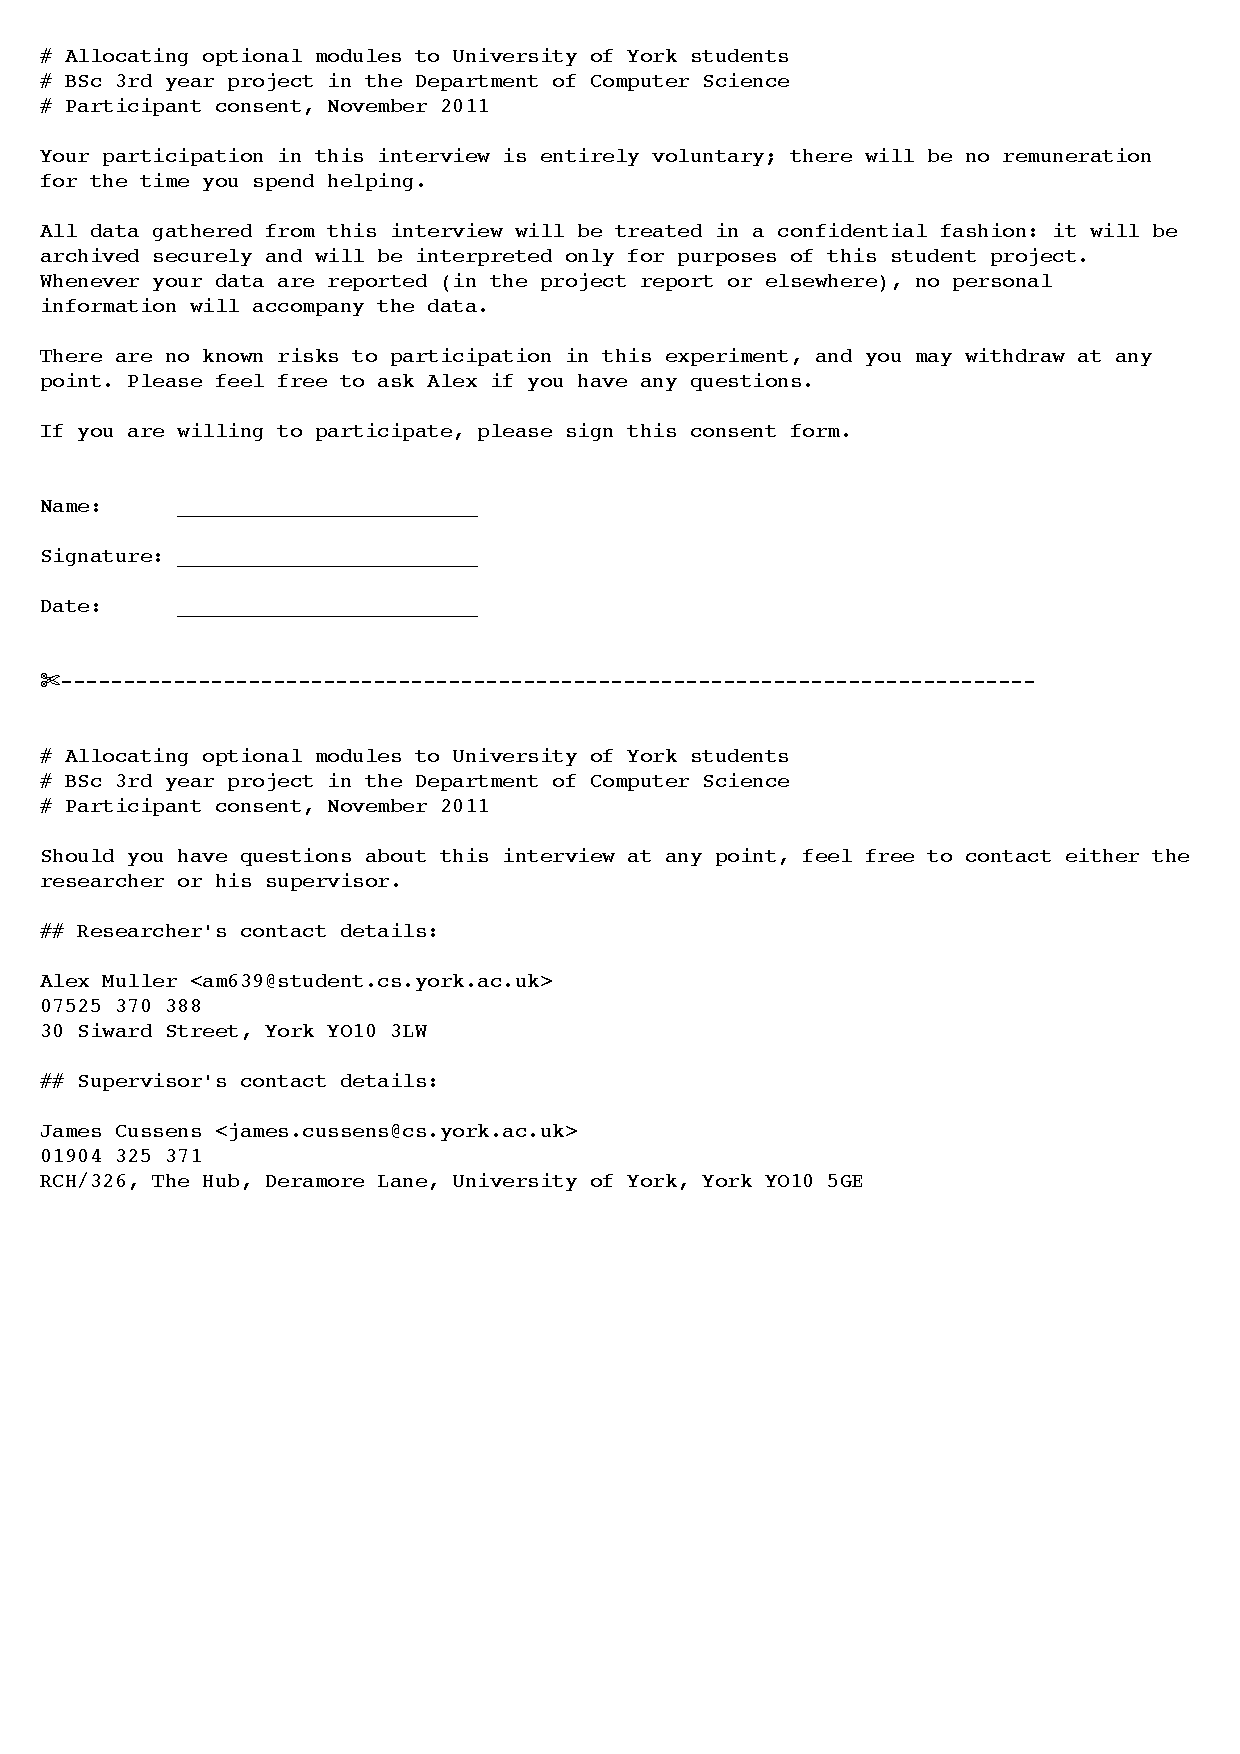
\includegraphics[width=140mm, trim=0 80mm 0 0]{images/consent.pdf}}
  \end{center}
  \caption{Participant consent form.}
  \label{participantconsent}
\end{figure}

\newpage
\bibliographystyle{references/IEEEtran.bst} % not just plain
\bibliography{references/references.bib}


\end{document}
